\section{Verteilungssicht}

\subsection{Infrastruktur-Übersicht}

Die Produktionsumgebung läuft in der Public Cloud von Microsoft Azure mit Kubernetes
als Orchestrierungsschicht. Alle Microservices werden als containerisierte Workloads
in einem Azure Kubernetes Service (AKS) Cluster betrieben. Die Datenhaltung erfolgt
über verwaltete Azure-Dienste (Azure Database for PostgreSQL), womit Betrieb,
Patching und Backup-Management an den Cloud-Provider delegiert werden.

\begin{figure}[H]
  \centering
  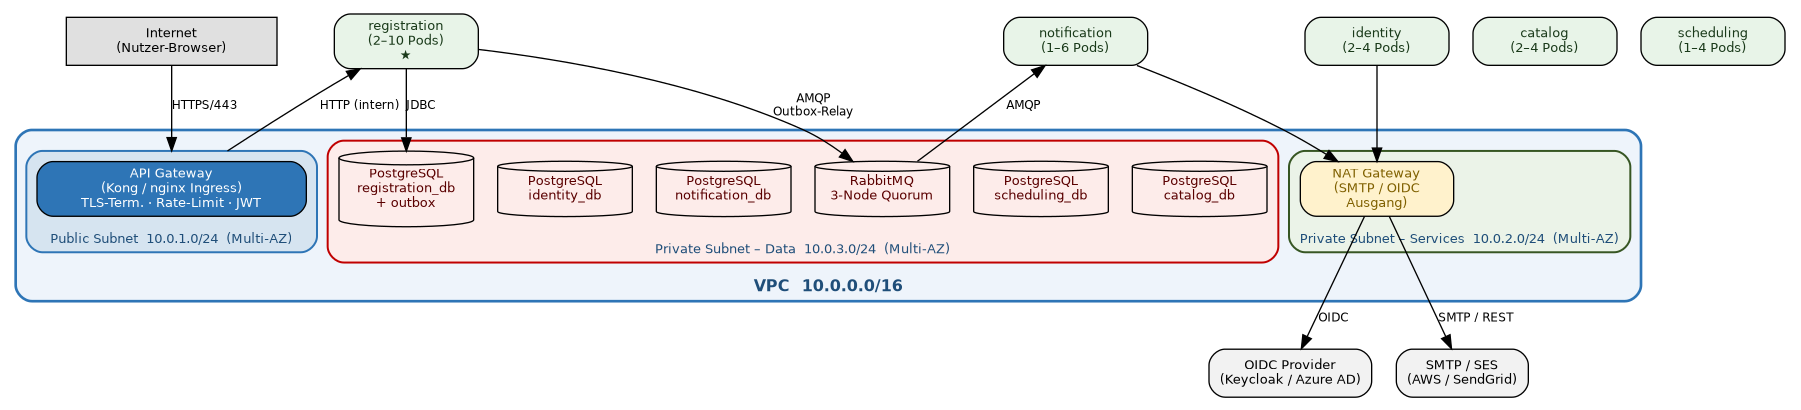
\includegraphics[width=\textwidth]{assets/deployment_diagram}
  \caption{\textit{Deployment-Diagramm: Netzwerk-Topologie (Kubernetes / Azure)}}
  \label{fig:deployment_diagram}
\end{figure}

\subsubsection{Cloud-Provider-Entscheid (ADR-010)}

Der Entscheid fiel zugunsten von \textbf{Microsoft Azure} (ADR-010). Ausschlaggebend waren:

\begin{itemize}
  \item \textbf{DSGVO-Compliance}: Azure-Regionen \textit{Switzerland North} (Zürich) und
  \textit{Switzerland West} (Genf) gewährleisten Datenresidenz in der Schweiz und
  erfüllen die Anforderungen gemäss DSG / DSGVO.
  \item \textbf{Managed Services}: Azure Database for PostgreSQL Flexible Server bietet
  automatisches Failover, PITR und integriertes Monitoring ohne Eigenaufwand.
  \item \textbf{Vendor Lock-in}: Minimiert durch den Einsatz cloud-agnostischer Technologien
  (Kubernetes, PostgreSQL, RabbitMQ) -- ein Anbieterwechsel bleibt möglich (vgl.\ R7).
  \item \textbf{Team-Kenntnisse}: Bestehendes Know-how im Betriebsteam mit Azure-Diensten
  reduziert den Einarbeitungsaufwand und das operative Risiko.
\end{itemize}

\subsection{Deployment-Umgebungen}

Das System durchläuft vier klar voneinander getrennte Umgebungen -- von der lokalen
Entwicklung bis zum produktiven Betrieb. Jede Umgebung ist auf ihren Zweck
zugeschnitten und wird über dieselbe CI/CD-Pipeline versorgt.

\begin{tabularx}{\textwidth}{L{2.5cm} L{2.5cm} X}
  \rowcolor{tableheader}
  \color{white}\textbf{Umgebung} & \color{white}\textbf{Plattform} & \color{white}\textbf{Beschreibung} \\
  Development & Docker Compose & Lokal; alle Services; vereinfachte Konfiguration (kein TLS, lokale DB). Hot-Reload. \\
  \rowcolor{tablegrey}
  Testing & K8s Namespace & Automatisch via CI/CD provisioniert; ephemeral -- nach Tests abgebaut. \\
  Staging & AKS Cluster & Produktionsähnlich; Abnahmetests; anonymisierte Prod-Daten. \\
  \rowcolor{tablegrey}
  Production & AKS Cluster (Multi-AZ) & HPA; automatische Failover-Mechanismen; Blue-Green-Deployment. \\
\end{tabularx}

\subsection{Infrastrukturkomponenten}

Die folgende Tabelle zeigt alle eingesetzten Infrastrukturkomponenten mit ihrer
konkreten Technologiewahl und Konfiguration. Die Kombination aus verwalteten
Azure-Diensten und cloud-agnostischen Open-Source-Technologien minimiert den
Betriebsaufwand bei gleichzeitig geringem Vendor Lock-in.

\begin{tabularx}{\textwidth}{L{3.2cm} L{3cm} X}
  \rowcolor{tableheader}
  \color{white}\textbf{Komponente} & \color{white}\textbf{Technologie} & \color{white}\textbf{Konfiguration} \\
  API Gateway & NGINX Ingress Controller & TLS-Terminierung, Rate-Limiting, JWT-Weiterleitung an Services;
  alternativ Spring Cloud Gateway für reaktive Routing-Logik \\
  \rowcolor{tablegrey}
  Orchestrierung & Azure Kubernetes Service~1.28+ & HPA, Readiness-/Liveness-Probes, Pod Disruption Budgets,
  Azure Monitor Integration \\
  Datenbanken & Azure Database for PostgreSQL~15 Flexible Server & Je Service eine Instanz (Database-per-Service);
  PITR~7~Tage; automatische Backups; Failover $<$~60~Sek. \\
  \rowcolor{tablegrey}
  Message Broker & RabbitMQ~3.12 & 3-Node-Quorum-Cluster; persistente Queues; DLQ; Management-UI
  über internen Ingress \\
  Monitoring & Prometheus + Grafana & RED-Pattern (Rate, Errors, Duration); Alerting bei
  Error-Rate~$>$~1\,\% und Latenz~$>$~500~ms (p99) \\
  \rowcolor{tablegrey}
  Logging & ELK-Stack & Strukturierte JSON-Logs; Correlation-ID über alle Services;
  30~Tage Retention; Index-Rotation täglich \\
  Tracing & OpenTelemetry + Jaeger & Distributed Tracing End-to-End; Sampling-Rate 10\,\%
  in Production, 100\,\% in Staging \\
  \rowcolor{tablegrey}
  CI/CD & GitHub Actions & Pipeline: Build $\to$ Unit-Tests $\to$ Integration-Tests $\to$
  Docker-Image $\to$ AKS-Deploy; automatisches Rollback bei fehlgeschlagenen Probes \\
  Secret Management & Azure Key Vault & Zentrales Secret-Management; Secrets werden zur
  Laufzeit per CSI-Treiber in Pods gemountet \\
\end{tabularx}

\subsection{Disaster Recovery Plan}

Der DR-Plan definiert verbindliche Zielwerte für Wiederherstellungszeit (RTO) und
maximal tolerierbaren Datenverlust (RPO)\footnote{RTO (Recovery Time Objective):
maximale Zeitspanne bis zur Wiederherstellung. RPO (Recovery Point Objective):
maximaler tolerierter Datenverlust in Zeit; RPO = 0~min bedeutet kein Datenverlust.}
je Infrastrukturkomponente. Die Massnahmen sind auf automatisches Failover ausgerichtet
-- manuelle Eingriffe bleiben auf Ausnahmefälle beschränkt.

\begin{tabularx}{\textwidth}{L{3cm} C{1.8cm} C{1.8cm} X}
  \rowcolor{tableheader}
  \color{white}\textbf{Komponente} & \color{white}\textbf{RTO} & \color{white}\textbf{RPO} & \color{white}\textbf{Strategie} \\
  PostgreSQL & 15~min & 5~min & Auto-Failover zu Read Replica; PITR~7~Tage; wöchentliche Restore-Tests (So, 03:00~UTC). \\
  \rowcolor{tablegrey}
  RabbitMQ & 5~min & 0~min & 3-Node Quorum-Cluster; kein Datenverlust. \\
  AKS Cluster & 30~min & N/A & Multi-AZ; Pod Disruption Budgets; Azure Availability Zones. \\
  \rowcolor{tablegrey}
  Application & 2~min & N/A & Blue-Green-Deployment; Liveness-Probes; automatisches Rollback. \\
\end{tabularx}

\begin{reviewbox}[DR-Testverantwortung]
  Der DR-Plan auf Systemebene wird halbjährlich als vollständiger Failover-Test in der Staging-Umgebung
  durchgeführt. Verantwortung: IT-Leiter (Patrick Hari). Protokoll geht an den CISO (Andrea Senn) für
  die Compliance-Dokumentation.
\end{reviewbox}

\subsection{Netzwerk-Topologie}

Das Netzwerk wird in drei Zonen aufgeteilt, die dem Prinzip der minimalen Exposition
folgen: Eingehender Verkehr läuft ausschliesslich über das öffentliche Subnet mit
NGINX Ingress; alle Microservices und Datenbankinstanzen sind in privaten Subnetzen
ohne direkten Internetzugang betrieben. Ausgehende Verbindungen der Services --
etwa für E-Mail-Versand oder OIDC -- werden über ein zentrales NAT Gateway\footnote{%
NAT Gateway (Network Address Translation): übersetzt private IP-Adressen der Services
auf eine öffentliche IP-Adresse für ausgehende Verbindungen -- ohne eingehenden
Zugriff aus dem Internet zu erlauben.} geführt.

\begin{tabularx}{\textwidth}{L{3.5cm} L{3.5cm} X}
  \rowcolor{tableheader}
  \color{white}\textbf{Netzwerkzone} & \color{white}\textbf{CIDR} & \color{white}\textbf{Beschreibung} \\
  VNet & 10.0.0.0/16 & Gesamtes Azure Virtual Network \\
  \rowcolor{tablegrey}
  Public Subnet & 10.0.1.0/24 (Multi-AZ) & NGINX Ingress / API Gateway -- einziger öffentlicher
  Zugangspunkt; Azure DDoS Protection Standard \\
  Private (Services) & 10.0.2.0/24 (Multi-AZ) & Alle Microservices -- kein direkter Internet-Zugang;
  Network Policies zwischen Services aktiv \\
  \rowcolor{tablegrey}
  Private (Data) & 10.0.3.0/24 (Multi-AZ) & PostgreSQL-Instanzen und RabbitMQ --
  nur aus Service-Subnet erreichbar; Private Endpoints \\
  NAT Gateway & Azure NAT Gateway & Ausgehende Verbindungen der Services (SMTP via
  SendGrid, OIDC-Endpunkte) \\
\end{tabularx}